\documentclass[a4paper,11pt]{article}
\usepackage[a4paper,left=3.1cm,right=3.1cm,top=3cm,bottom=2.9cm]{geometry}
\usepackage[english]{babel}
\usepackage[utf8]{inputenc}
\usepackage{amsmath,amsthm,amssymb,amsfonts,stmaryrd, wasysym}
\usepackage{color}
\usepackage{graphicx}
\usepackage{todonotes}
\usepackage{subcaption}
\usepackage{wrapfig}
\usepackage{multirow} %multirow in table

\usepackage{algorithm}
\usepackage{algpseudocode}
\usepackage{xcolor}
\usepackage{titling}
\usepackage{caption}
\usepackage{hyperref}
\captionsetup{font=footnotesize}

\newcommand{\subtitle}[1]{%
  \posttitle{%
    \par\end{center}
    \begin{center}\large#1\end{center}
    \vskip0.5em}%
}

%%%%%%%%%%%%%%%%% Kopf- & Fußzeile %%%%%%%%%%%%%%%%%
\usepackage[footsepline]{scrlayer-scrpage}
\pagestyle{scrheadings}
\clearscrheadfoot
\title{Machine Learning - Exercise 3}
\subtitle{Model Stealing/Extraction}
\author{Christian Hatschka, Daniel Fangl, Esra Ceylan}
\date{February 2021}
\ihead{\thetitle}
\ifoot{\newline \theauthor}
\ofoot{\newline \pagemark}
\setlength{\headheight}{15pt}
\setlength{\footheight}{29pt}

\begin{document}
\maketitle

\section{Group members}
    Daniel Fangl (01526097) has a bachelor in Software Engineering and is currently in the master course Software Engineering and Internet Computing. Christian Hatschka (01525634) and Esra Ceylan (01526801) both have a bachelor in Mathematics and are currently enrolled in the master course Logic and Computation.
    
\section{Introduction}
    As the construction of a good model is an expensive and time consuming task, the thought of training a model based on an existing but not explicitly given one is interesting. We will do this using the original model as a black-box and taking its predictions into account.
    
    The aim of this project is to extract several models by using different model-stealing methods. Moreover, we will test their efficiency and accuracy and compare their performance to the performance of the underlying original model.
    
\section{Copycat Networks for CNN}
    This model stealing attack was proposed by Correia-Silva et al.~\cite{copycat} and aims to copy a Convolutional Neural Network. First, we will use the target CNN as a black-box to label our training set, which can also contain instances from the non-problem domain if the model allows us to classify them. For example the Microsoft Azure Emotion API does not allow to upload instances, where it cannot detect a face, hence which are not part of the problem-domain. Even images containing a face can sometimes be rejected as the API could not always detect a face. By classifying the data we create a fake dataset which will be used to train the extracted model.
    
    Next, we select a model architecture of the copycat network. A possible problem with this approach is that we might not know the model architecture of the original network. However, this should not be a big problem as the knowledge can be copied to a different model.
    As pre-trained models tend to perform better, we used the VGG-16 architecture with pre-trained weights. It is obviously optimal if the pre-trained model is already close to the problem domain. In the next step we use the generated dataset to fit the pre-trained model.
    
    As described in~\cite{copycat} we will use Stochastic Gradient Descent with a Step Down policy for the learning rate for training the copycat model. 
    
    \subsection{First Data set}
        As our first data set we combined the data sets described in the following two subsections. 
        %Since KDEF and AKDEF were one of the used data sets in the paper of Correia-Silva et al. we wanted to take them as validation that we achieve similar results. Unfortunately, they contain only about 5\,000 samples in total and we could not get access to other data sets used in the paper. Therefore, we combined them with a larger data set.
        Unfortunately, we could not get access to the data sets used in~\cite{copycat} to compare our results to the results in the paper. Therefore, we used different data sets and combined them to obtain a larger number of instances.
        
        \subsubsection{KDEF and AKDEF}
            The Karolinska directed emotional faces data set~\cite{kdef} (short KDEF) contains 4\,900 images of human facial expressions. The pictures were taken of 70 different people (35 male and 35 female) displaying 7 different emotional expressions. All people portrayed were amateur actors between the ages of 20 and 30 and had no facial hair, glasses or makeup during the photos. Each of the expressions were taken from multiple different angles. 
            
            The averaged Karolinska directed emotional faces data set~\cite{kdef} (short AKDEF) contains $70$ averaged images of KDEF. The averaging was done over images containing the same gender, angle and emotional expression.
            
            Both data sets contain labels and were made by the Karolinska Institute in Stockholm, Sweden by the Department of Clinical Neuroscience in 1998. The data sets have been used in a large number of research publications on the topic. 
            
        \subsubsection{Emotion Detection from Facial Expressions}
            This data set was taken from the Kaggle competition 'Emotion Detection From Facial Expressions'~\cite{kaggle-emotion}. 
            It contains 13\,690 images of human faces with different emotions. The data set was constructed from a variety of different sources, e.g.
            \begin{itemize}
                \item labeled Faces In The Wild,
                \item the Japanese Female Facial Expression (JAFFE) Database,
                \item indian Movie Face database (IMFDB),
                \item the Extended Yale Face Database B.
            \end{itemize}
            
            Additionally, this data set contains labeled data, like the previous set, allowing us also to compare the overall performance of the original model and the extracted one. 
    
    \subsection{Microsoft Azure Emotion API}
        As our first target model we chose the publicly available Microsoft Azure Emotion API. For an input image it returns a confidence across a set of emotions for each face in the image. 
        
        This API classifies the emotion a face portrays, in the form of a percentage vectors that assigns values to the following emotions:
            \begin{itemize}
                \item Anger
                \item Contempt
                \item Disgust
                \item Fear
                \item Happiness
                \item Neutral
                \item Sadness
                \item Surprise
            \end{itemize}
        For example the following face from the publicly available Karolinska Directed Emotional Faces (KDEF) dataset, returned a vector that assigned a percentage of $0.999$ to Happiness $0.001$ to Surprise and $0$ to everything else.
            \begin{figure}[h!]
                    \centering      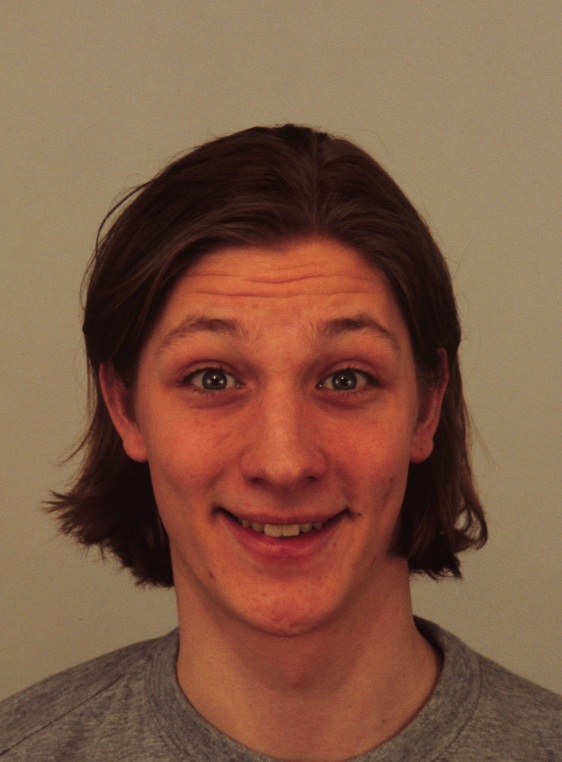
\includegraphics[scale=0.2]{exercise_3/paper/images/AM18HAS.JPG}
                    \caption{A face classified as happy by Azure}
                    \label{fig:Happy_face}
            \end{figure}
        
        There is a free pricing option as well as a premium plan. As Microsoft has a promotion for students, which gives 100€ of free credit, we chose the premium plan which allows us to submit up to 10 images per second.
        
        We started by stealing the model behind this API as it was already copied in the paper and as such we could assess whether the performance of our copied classifier was similar to the performance of the stolen classifier in the paper.
        
        Originally the plan was to add images, which are not part of the problem domain to the images to be classified by the blackbox, however as Azure does not classify images in which it does not recognise any faces, this was not possible.
        
        Testing the Azure Classifier using the prelabeled data from the Kaggled Competion we got an accuracy of $0.76$.
        
    \subsection{Evaluation 1}
        We used the Karolinska Directed Emotional Faces (KDEF) and Averaged Karolinska Directed Emotional Faces (AKDEF) dataset to query Azure as a Blackbox. As Azure did not recognise some of the faces we added No face detected as an additional class. \\
        
        The Cnn-Classifier was trained through by a Multi-layer perceptron. As the Copying algorithm used for this Classifier was rather basic we mapped the size of the training set to the size of the subset of AKDEF/KDEF used to train our copy-cat.\\
        
        In order to compare the performance of our copied classifier to the original we used the ..\todo[]{dataset}.
        
        \todo[]{graph}


    \subsection{Second Data Set}
        https://www.kaggle.com/crawford/cat-dataset 9000 Bilder 
        
        http://vision.stanford.edu/aditya86/ImageNetDogs/ 20 580 Bilder
        
        
    
\section{Classifier 2}


\section{Conclusions}

\bibliographystyle{abbrv}
\bibliography{literature}

\end{document}